\chapter{\IfLanguageName{dutch}{Stand van zaken}{State of the art}}
\label{ch:stand-van-zaken}

% Tip: Begin elk hoofdstuk met een paragraaf inleiding die beschrijft hoe
% dit hoofdstuk past binnen het geheel van de bachelorproef. Geef in het
% bijzonder aan wat de link is met het vorige en volgende hoofdstuk.

% Pas na deze inleidende paragraaf komt de eerste sectiehoofding.

%Dit hoofdstuk bevat je literatuurstudie. De inhoud gaat verder op de inleiding, maar zal het onderwerp van de bachelorproef *diepgaand* uitspitten. De bedoeling is dat de lezer na lezing van dit hoofdstuk helemaal op de hoogte is van de huidige stand van zaken (state-of-the-art) in het onderzoeksdomein. Iemand die niet vertrouwd is met het onderwerp, weet nu voldoende om de rest van het verhaal te kunnen volgen, zonder dat die er nog andere informatie moet over opzoeken \autocite{Pollefliet2011}.

%Je verwijst bij elke bewering die je doet, vakterm die je introduceert, enz. naar je bronnen. In \LaTeX{} kan dat met het commando \texttt{$\backslash${textcite\{\}}} of \texttt{$\backslash${autocite\{\}}}. Als argument van het commando geef je de ``sleutel'' van een ``record'' in een bibliografische databank in het Bib\LaTeX{}-formaat (een tekstbestand). Als je expliciet naar de auteur verwijst in de zin, gebruik je \texttt{$\backslash${}textcite\{\}}.
%Soms wil je de auteur niet expliciet vernoemen, dan gebruik je \texttt{$\backslash${}autocite\{\}}. In de volgende paragraaf een voorbeeld van elk.

%\textcite{Knuth1998} schreef een van de standaardwerken over sorteer- en zoekalgoritmen. Experten zijn het erover eens dat cloud computing een interessante opportuniteit vormen, zowel voor gebruikers als voor dienstverleners op vlak van informatietechnologie~\autocite{Creeger2009}.

% Te beschrijven in de stand van zaken
% Containers: Hoe werken ze en hoe worden ze gebruikt
% Docker: wat is het en waarvoor wordt het gebruikt?
% Container orkestratie: wat is het en waarom is het nodig
% Kubernetes: wat is het en waarvoor wordt het gebruikt?
% Security: veel voorkomende problemen, best practices
% Security tools: Welke zijn er en hoe werken ze
De stand van zaken of \textit{State of the art} geeft een algemeen beeld weer van de technologieën die worden overwogen in dit onderzoek en tevens de verschillend manieren van toepassing.

\section{Containers}
In dit hoofdstuk zal uitgelegd worden wat containers zijn, hoe ze werken en waarvoor ze worden gebruikt.

Containers bieden veel voordelen vergeleken met normale virtuele machines (VM's). Ze kunnen snel opgezet worden en zijn gemakkelijk om te configureren terwijl virtuele machines vaak groot en traag zijn. Containers zijn pakketten waarin een applicatie vervat zit, samen met zijn benodigde bibliotheken en afhankelijkheden. Hierdoor kunnen ze vlot van de ene omgeving naar de andere worden overgezet zonder dat er extra configuratie nodig is \autocite{Education2019}. Containers maken gebruik van besturingssysteem-virtualisatie om processen te isoleren van het \textit{host} besturingssysteem. Daarnaast controleert het tevens de CPU gebruik en hoeveelheid RAM geheugen van deze processen (Docker, 2018).

Containers hebben eigenlijk geen eigen besturingssysteem nodig, alle containers delen 1 gezamenlijke \textit{runtime engine}. Een \textit{runtime engine} is de laag die verantwoordelijk is voor de communicatie tussen het besturingssysteem van de host machine en de containers zelf. De meeste gebruikte runtime engine is de \textit{Docker Engine}\footnote{docs.docker.com/engine/}.

\subsection{Container vs. virtuele machine}
\subsubsection{Hypervisors}
Bij traditionele virtuele machines virtualiseert een \textit{hypervisor} de fysieke hardware. De hypervisor regelt het resource gebruik tussen de verschillende VM's en zorgt ervoor dat de hardware van de host (de fysieke hardware waar de hypervisor op geïnstalleerd is) eerlijk verdeelt wordt. Er zijn 2 types hypervisor \autocite{VMWare2021}, namelijk:
\begin{itemize}
    \item Type 1: Ook wel \textit{bare metal} hypervisors genoemd. Deze werken rechtstreeks op de fysieke hardware van de host en hebben dus geen onderliggend besturingssysteem nodig. Door het rechtstreekse contact tussen de hypervisor en de hardware wordt een type 1 hypervisor beschouwd als de best presterende en meest efficiënte hypervisor. Een type 1 hypervisor wordt ook beschouwd als het veiligste van de 2, dit omdat de gebreken en kwetsbaarheden die doorgaans in besturingssystemen aanwezig zijn hier onmogelijk zijn.
    \item Type 2: Ook wel \textit{hosted} hypervisors genoemd. Deze worden doorgaans geïnstalleerd op een bestaand besturingssysteem en steunt daar ook op voor het beheren van de resources. Een groot voordeel van type 2 hypervisors is dat ze een breed gamma aan hardware ondersteunen.
\end{itemize}
\begin{figure}[ht]
    \centering
    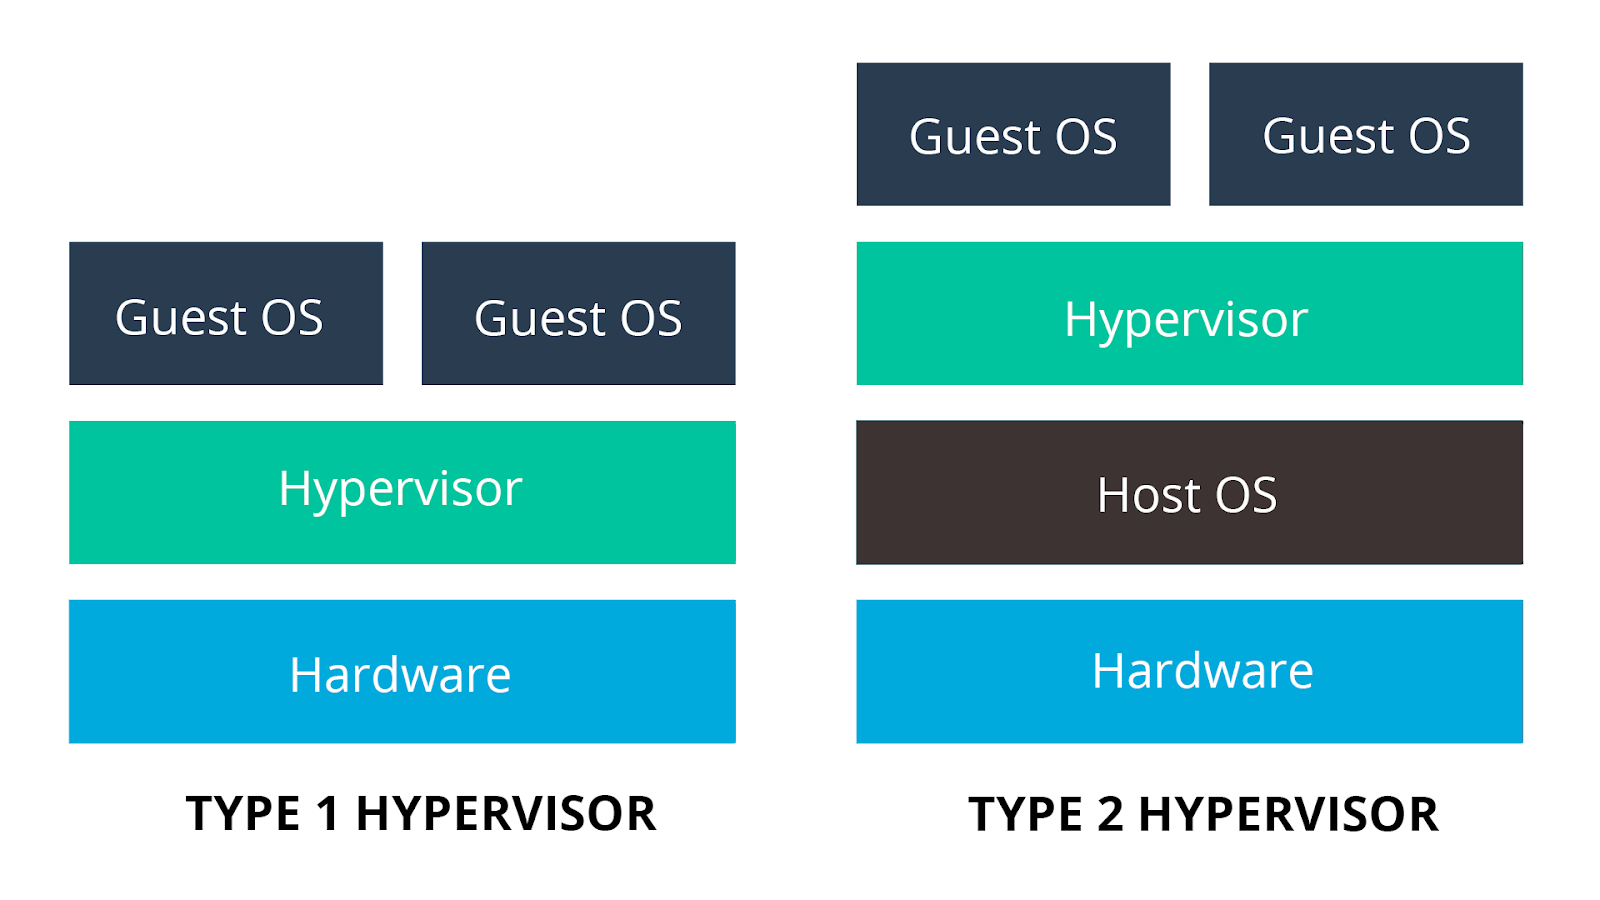
\includegraphics[width=\linewidth]{img/Hypervisor.png}
    \caption{Type 1 \& Type 2 Hypervisor \autocite{VMWare2021}}
    \label{fig:hypers}
\end{figure}

Tegenwoordig zijn type 1 hypervisors de meest gebruikte in productieomgevingen vanwege het efficiente resource gebruik en veiligheid. Type 2 hypervisors worden dan meer gebruikt voor testomgevingen omdat ze gemakkelijker op te zetten zijn.

Elke VM heeft zijn eigen volwaardig besturingssysteem, wat ervoor zorgt dat ze zeer veel resources gebruiken en vaak traag zijn. In plaats van de onderliggende hardware te visualiseren gebruiken containers het besturingssysteem (meestal is dit Linux) zelf, zo bevat elke individuele container enkel de applicatie en de bijhorende bibliotheken en afhankelijkheden bevat \autocite{Education2020}.

\begin{figure}[ht]
    \centering
    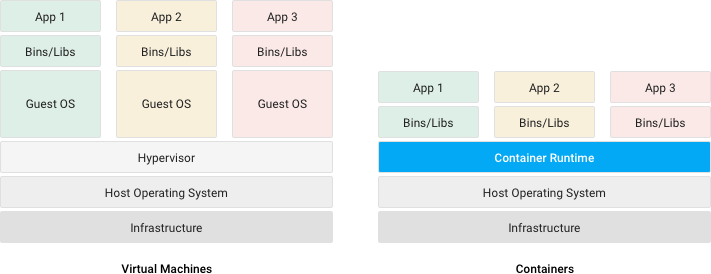
\includegraphics[width=\linewidth]{img/container-vs-vm.png}
    \caption{Container vs. virtuele machine \autocite{Google2016}}
    \label{fig:example}
\end{figure}


\subsection{Waarvoor worden containers gebruikt}
Containers zijn zeer veelzijdig en kunnen dus in veel verschillende omstandigheden gebruikt worden. Enkele \textit{use cases} waarvoor containers zeer geschikt zijn \autocite{Docker2021}:

\begin{itemize}
  \item \underline{Microservices}: Containers zijn klein en licht, waardoor ze goed passen bij microservice-architecturen waarin applicaties zijn opgebouwd uit vele, losjes gekoppelde en onafhankelijk services.
  \item \underline{Modernisering en migratie van applicaties}: Een van de meest voorkomende benaderingen voor het moderniseren van applicaties begint met het containeriseren ervan, zodat ze naar de \textit{cloud} kunnen worden gemigreerd.
  \item \underline{Nieuwe ontwikkelaars snel inwerken}: Door gebruik te maken van containers verloopt het opzetten van een nieuwe lokale ontwikkelingsomgeving snel en vlot, hierdoor kunnen de ontwikkelaars direct aan de slag.
\end{itemize}


\section{Docker}
\textit{Docker}\footnote{docker.com/} is een open source container platform dat sinds de release in 2013 ongelofelijk populair is geworden. In november 2019 stond de teller van aantal \textit{pulls} op de \textit{Docker hub} op 130 miljard,  in juli 2020 stond deze al op 242 miljard. Dat is bijna dubbel op minder dan 8 maand tijd \autocite{Kreisa2020}. Docker-containers kunnen overal draaien, in een het datacenter, bij een externe serviceprovider of in de cloud. Docker containers kunnen zowel op Linux als op Windows draaien. Containers die op Windows gebaseerd zijn kunnen echter alleen op Windows systemen draaien, maar Linux containers kunnen op zowel Linux systemen en Windows systemen draaien (met behulp van een Linux VM). Dit komt omdat containers ontworpen zijn om het besturingssysteem van de host te gebruiken \autocite{Anil2018}.


\subsection{Hoe werkt docker}
Docker gebruikt een \textit{Client-Server} architectuur. Deze werkt als volgt: De Docker \textit{Client} communiceert met de Docker \textit{Deamon} (een proces dat op de achtergrond draait en bepaalde (onderhouds)taken uitvoert). Deze is verantwoordelijk voor het bouwen, runnen en verspreiden van containers \autocite{Docker2021a}.

\subsection{Docker componenten en terminologie}

\subsubsection{Docker Deamon}De Docker Daemon (\verb|dockerd|) luistert naar Docker Application programming interface (API) verzoeken en beheert Docker objecten zoals \textit{images}, \textit{containers}, netwerken, en \textit{volumes}.

\subsubsection{Docker Client}De Docker Client is de meest gebruikte manier voor gebruikers om te communiceren met Docker. De client stuurt alle ingevoerde commando's (zoals \verb|docker pull| en \verb|docker run|) door naar de Docker Daemon die deze uitvoert.

\subsubsection{Docker registries}Een \textit{Docker register} is een bibliotheek die \textit{Docker images} opslaat. De standaar register voor Docker is de \textit{Docker Hub}\footnote{hub.docker.com/}. Als de Docker daemon geen lokale Docker image vindt gaat deze standaard in de \textit{Docker Hub} zoeken. Wanneer het \verb|docker pull| of \verb|docker run| commando's wordt gebruikt, worden de benodigde images uit het register gehaald.
\subsubsection{Docker objecten}Docker maakt gebruik van images, volumes en netwerken, al deze onderdelen worden objecten genoemt. Volgens \textcite{Docker2021a} zijn dit de belangrijkste objecten:

\begin{itemize}
        \item \textbf{Images}: Docker images zijn read-only sjablonen met instructies om een Docker container op te zetten. Docker images kunnen uit de Docker hub gehaald worden en direct gebruikt worden zonder verdere configuratie, of je kan bijkomende instructies toevoegen aan de \textit{base image} en deze opslaan als een nieuwe en aangepaste Docker image. Een Docker image is vaak gebaseerd op een andere images (i.e., Een nieuwe image kan gebaseerd zijn op een bestaande \textit{Ubuntu} image maar installeert en configureert ook een \textit{Apache} webserver). Alsook is het mogelijk om zelf een compleet nieuwe image te maken met behulp van een \textit{dockerfile}.
        \item \textbf{Containers}: Een container is een uitvoerbare instantie van een image die wordt gecontroleerd via de Docker API. Een container kan verbonden worden met andere containers, verbonden worden aan opslag of gebruikt worden als basis voor nieuwe image.
        \item \textbf{Volumes}: De persistente gegevens die Docker containers kunnen gebruiken wordt opgeslagen in zogenaamde volumes. Deze volumes worden volledig gecontroleerd via de Docker API en bevinden zich buiten de container zelf. Hierdoor blijft het gewicht van de containers laag en kan de data blijven bestaan ook al wordt de container gestopt of verwijderd.
\end{itemize}

\section{Container orkestratie}
Container orkestratie helpt bij het opzetten, beheren, schalen en verbinden van een grote hoeveelheid containers. Container orkestratie helpt dus om complexe procedures te vergemakkelijken. Dit door veelvoorkomende processen en werkstromen te stroomlijnen en te optimaliseren. Nog een belangrijk onderdeel van orkestratie is het geautomatiseerd onderhoud van de applicaties die in de containers draaien \autocite{RedHat2021}.

\subsubsection{Waarvoor word container orkestratie gebruikt?}

Container orkestratie wordt vooral gebruikt voor het automatiseren en beheren van, onder andere, de configuratie en uitrol, het toewijzen van resources, de \textit{Load balancing} en het monitoren van containers.
%Container orkestratie wordt vooral gebruikt voor het automatiseren en beheren van:
%\begin{itemize}
%    \item De configuratie en uitrol van containers.
%    \item De toewijzing van resources.
%    \item De \textit{Load balancing} op basis van de belasting van het systeem.
%    \item Het monitoren van containers.
%    \item De beveiliging van interacties tussen containers.
%\end{itemize}

\subsection{Container orkestratie tools}
Om aan container orkestratie te gaan doen zijn er natuurlijk tools nodig die ons alle nodig functionaliteiten kunnen aanbieden. \textcite{DevopsCube2021} geeft een overzicht van de meest prominente orkestratie tools.

\subsubsection{Kubernetes}
Kubernetes(k8s)\footnote{kubernetes.io/} is een open-source, container cluster manager en orchestratie tool. Het is gebouwd met een uitstekende resource manager voor het inzetten van containers op een efficiëntere manier. Kubernetes is voor vele organisaties de de facto container orkestratie tool geworden voor veel organisaties. Volgens \textcite{CNCF2021} zijn er meer dan 109 tools om containers te beheren, maar 89\% is gebouwd met k8s aan de basis.

\subsubsection{Openshift}
Openshift is een van die 89\% tools die gebouwd zijn bovenop Kubernetes. Het Openshift-project\footnote{openshift.com/} word onderhouden door RedHat\footnote{redhat.com/}. Het heeft zowel een open source versie (\textit{openshift origin}\footnote{github.com/openshift/origin}) als een enterprise versie (\textit{openshift container platform}\footnote{openshift.com/products/container-platform}).

\subsubsection{Hasicorp Nomad}
Nomad\footnote{nomadproject.io/} is een orkestratieplatform van Hashicorp\footnote{hashicorp.com/} dat containers op schaal kan ondersteunen. Op het vlak van applicatiemanagement is het zeer sterk vergelijkbaar met Kubernetes. Echter het feit da Nomad ook niet-containerapplicaties kan beheren zorgt ervoor dat het zich toch kan distantiëren van de andere orkestratie tools. Nomad kan ook feilloos geïntegreerd worden met andere tools van Hashicorp.

\section{Kubernetes}
Hier zal uitgelegd worden wat k8s is en hoe het werkt, ook de verschillende technische termen die eigen zijn aan k8s zullen uitgelegd worden.

\section{Security}
Hier word het security aspect van containers en container orkestratie besproken. (redelijk high level want kan ongeloofelijk complex worden)

\subsection{Meest voorkomende security problemen}
Hier worden de meest voorkomende security problemen opgelijst en worden ze kort besproken (Techinsche uitleg over hoe deze problemen onstaan)

\subsection{Hoe een container cluster beveiligen}
Uitleg over hoe een container cluster beveiligt kan worden (Best practices en security tools) + uitleg over ingebouwde security features.

\section{Security tools}
Hier worden enkele security tools opgeslijst en hun werking kort besproken.